\documentclass[14pt]{extarticle}
\usepackage{extsizes}
\usepackage[utf8]{inputenc}
\usepackage[russian]{babel}
\usepackage{amssymb}
\usepackage{amsmath}
\usepackage{enumitem}
\usepackage{color}
\usepackage{tabu}
\usepackage{graphicx}
\usepackage{grffile}
\usepackage{float}
\usepackage[top=2.5cm, bottom=2.5cm, left=2.5cm, right=2.5cm]{geometry}
\setlist{nolistsep}
\setcounter{tocdepth}{3}
\setcounter{secnumdepth}{3}
\setlength{\parskip}{0.7em}
\setlength{\parindent}{0em}

\begin{document}

\thispagestyle{empty}
{\centering Московский государственный университет имени М.В. Ломоносова \\}
{\centering Механико-математический факультет \\}
{\centering Кафдра вычислительной математики \\}
\begin{figure}[H]
\centering
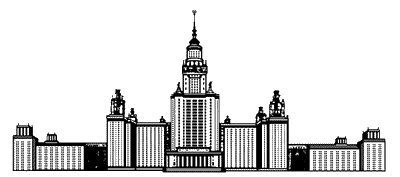
\includegraphics[width=0.4\linewidth]{imgs/msu.png}
\end{figure}
\vspace*{0.5cm}
{\centering Дипломная работа \\}
\vspace*{1.5cm}
{\centering \textbf{\large Применение задачи классификации для разделения
области, заданной набором космических снимков, на регионы, обладающие почвенной
интерпретацией} \\}
\vspace*{1.5cm}
\begin{flushright}
\textbf{Работу выполнил \\}
студент 610 группы \\
Рухович Данила Дмитриевич \\
\vspace*{0.5cm}
\textbf{Научный руководитель \\}
д.ф.-м.н., профессор \\
Васенин Валерий Александрович \\
\end{flushright}
\vspace*{4.5cm}
{\centering Москва \\ 2017 \\}

\newpage

\tableofcontents
\newpage

\section{Введение.}

\par
В последние годы в связи с появлением в открытом доступе множества космических снимков стала
актуальной задача автоматического распознавания объектов на этих коллекциях. В частности,
в почвоведении исследуют разрешимость задачи разделения поверхности Земли на регионы,
обладающие почвенной интерпретацией. Под этим подразумевается широкий набор задач: 
определение засоленности почв \cite{salt-1}, \cite{salt-2}, 
определение влияния типа почв на вегетационный
индекс территорий \cite{soil-line-2}, классификация территорий по типам почв. 
Именно для задаче автоматического разделения территорий по типам почв до сих пор не найдено
приемлимых на практике решений. В работе \cite{soil-line-1} авторы исследуют применимость
модели линии почвы к выделению голой почвы и классификации её типов по одному космическому снимку
и получают хорошее качество выделения, однако разделение области по типам почв дано лишь 
приблизительное и без математических оценок. В статье \cite{soil-line-3} описано разделение
2 типов почв по 1 спутниковому снимку и показано, что добиться хорошей точности не удается.
В еще одной недавней работе \cite{soil-line-6} авторы применяют линейную классификацию 185
точек 1 космического снимка на 16 почвенных классов и достигают точности менее 50\%,
для 7 почвенных классов получают точность 52\%. Однако в работах не предлагаются методы
переноса моделей на другие территории и проверка результатов скользящим контролем или по 
отложенной выборке.
\par
В данной работе предложен новаторский метод решения задачи классификации точек поверхности
по типам почв, показывающий сильно лучшие метрика качества, чем все предыдущие. Для решения
задачи используются современные методы машинного обучения, а так же вводятся алгоритмы,
позволяющие использовать набор разновременных снимков одной территории для признакового 
описания объектов.

\section{Постановка задачи.}


\subsection{Постановка задачи классификации.}

\par
Напомним определение задачи классификации. 
Пусть $\mathcal{X}$ - множество описаний объектов, 
$\mathcal{Y}$ - конечное множество меток классов, и 
существует неизвестная целевая зависимость - отображение 
$y^\star:\ \mathcal{X} \to \mathcal{Y}$, 
значения которой известны только на конечном подмножестве объектов
$x_1, ..., x_n \in X$. Пары объектов и ответов $(x_i, y_i)$ называют прецендентами.
Совокупность таких пар ${(x_i, y_i)}_{i=1}^n$ называют обучающей выборкой.
\par
Задача обучения по прецендентам заключается в восстановлении зависимости $y^\star$
по заданной обучающей выборк, т.е. в построении решающей функции 
$\mathcal{X} \to \mathcal{Y}$, которая бы
приближала целевую функцию $y^\star(x)$ причем не только на объектах обучающей выборки,
но и на всем множестве $\mathcal{X}$. Кроме того, решающая функция должно допускать эффективную
реализацию на вычислтельой системе.
\par
Каждый объект $x_i$ задается измерениями своих характеристик $f_j(x_i)$, 
которые называют признаками. Таким образом, признаковое описание задается набором функций
$f_j:\ \mathcal{X}\to D_{f_j}$, где $D_{f_j}$ - множество допустимых значений признака.
Выделяют несколько типов признаков в зависимости от множества $D_f$:
\begin{itemize} 
    \item бинарный - $D_f=\{0,1\}$
    \item номинальный - $D_f$ - конечное множество,
    \item порядковый - $D_f$ - конечное упорядоченной множество,
    \item количественный - $D_f$ - множество действительных чисел.
\end{itemize}
Пусть признаков $m$ штук, тогда признаковым описание каждого объекта 
$x_i \in \mathcal{X}$ служит вектор $(x_i^1, ..., x_i^m)$. 
Таким образом обучающая выборка представляется в виде совокупности матрицы 
$X \in \mathbb{R}^{n \times m}$ и вектора $Y \in \{1, ..., k\}^n$, где 
$k$ - количество классов.

\subsection{Постановка задачи классификации типов почв по космическим снимкам.}

\par
Основной целью данной работы является решение задачи пространственной классификации
по типам почв некоторой территории, заданной набором её космических снимков.
\par
Как было покаано в предыдущем разделе, входными параметрами задачи классификации являются
признаковое пространство объектов, множество меток классов и обучающая выборка выборка,
составленная из пар элементов данных двух множеств. В качестве объектов рассматриваются точки
поверхности Земли, заданные георграфическими координатами. Признаковое пространство определеяется
из данных космических снимков, покрывающих исследуемую территорию. Метки классов берутся
из результатов наземных исследований территории почвоведами.
\par
В данной работе также исследуется информативность некоторых признаков и моделей, 
которые могут быть использованы не только для задачи классификации, 
но и для других приложений из области почвоведения. 
Подробнее об этом - в опубликованных автором работах \cite{rukhovich-1}, \cite{rukhovich-2},
\cite{rukhovich-3}.

\section{Предлагаемое решение.}


\subsection{Классификационные модели.}


\subsubsection{Метод ближайших соседей.}

\par
Метод взвешенных $k$ ближайших соседей - это метрический алгоритм классификации,
основанный на оценивании сходства объектов. Классифицируемый объект относится к тому классу,
к которому принадлежат ближайшие к нему объекты обучающей выборки. Более формально,
пусть на множестве объектов задана функция расстояния $\rho$, например, евклидова:
\[
    \rho(x, x') = \sum_i (x_i - x_i')^2.
\]
Для произвольного объекта $x \in \mathcal{X}$ расположим $k$ его ближайших соседей
из обучающей выборки в порядке возрастания расстояния до 
$x: \rho(x, x_{1;x}) \le \rho(x, x_{2;x}) \le ... \rho(x, x_{k;x})$.
Тогда формула для классификатора будет иметь вид:
\[
    A(x)=\arg\max_{y\in\mathcal{Y}} \sum_{i=1}^k[y_{i;x}=y]w(i, x),
\]
где $w(i, x)$ - заданная весовая функция, оценивающая важность $i$-ого соседа для
классификации объекта $x$. Существует множество эвристик для определения типа $w$,
самые простые из которых это: константная и обратно пропорциональная расстоянию до $i$-ого
объекта. Параметр $k$ данного метода подбирается для каждой задачи индивидуально.

\subsubsection{Случайный лес.}

\par
Бинарное решающее дерево (Decision tree) - это алгоритм классификации, задающийся бинарным
деревом, в котором каждой внутренней вершине $v \in V$ приписан предикат 
$\beta_v:X\to\{0, 1\}$, а каждой терминальной вершине $v \in V$ приписано имя класса 
$y_v \in Y$. При классификации объекта $x \in \mathcal{X}$ он проходит по предикатам
пусть от корня дерева к одному из листьев, и результатом является метка класса этого листа.
\par
Объект $x$ доходит до вершины $v$ тогда и только тогда, когда выполняется конъюнкция
$K_v(x)$, составленная из всех предикатов, приписанных внутренним вершинам дерева
на пути от корня $v_0$ до $v$. Пусть $T$ - множество всех терминальных вершин дерева. 
Множества объектов $\Omega_v=\{x \in \mathcal{X} : K_v(x)\}$, выделяемые терминальными
конъюнкциями вершин $v \in T$, попарно не пересекаются, а их объединение совпадает
со всем пространством $\mathcal{X}$. Тогда получаем формулу алгоритма классификации:
\[
    a(x) = \arg\max_{y \in Y} \sum_{v \in T,\ c_v=y} K_v(x).
\]
\par
Существует множество эвристик для построения решающего дерева, т.к. поиск оптимального - 
NP полная задача. Основными параметрами, подбираемыми под каждую задачу являются
критерий разбиения вершины и ограничение его высоты.
\par
Случайный лес (Random Forest) является композицией решающих деревьев. Все деревья строятся
случайно и независимо, затем для каждого объекта устраивается голосование среди
предсказаний каждого дерева. Соответственно, ответом является класс, за который голосуют
большинство деревьев.

\subsubsection{Метод опорных векторов.}

\par
Метод SVM (Support vector machine) позволяет разделить объекты двух классов
гиперплоскостью $wx-b=0$ с максимальным отступом между ней и классами.
Вектор $w$ - перпендикуляр к разделяющей гиперплоскости.
Параметр $b$ равен по модулю расстоянию от гиперплоскости до начала координат.
В случае линейной разделимости опорными векторами будут являться ближайшие
к гиперплоскости точки.
Плоскости, параллельные разделяющей и проходящие через опорные вектора классов,
задаются уравнениями $wx-b=1$ и $wx-b=-1$, см. рис. \ref{image:svm_linear}.
Ширина максимизируемой полосы между ними равна $\frac{2}{||w||}.$
\begin{figure}[H]
\centering
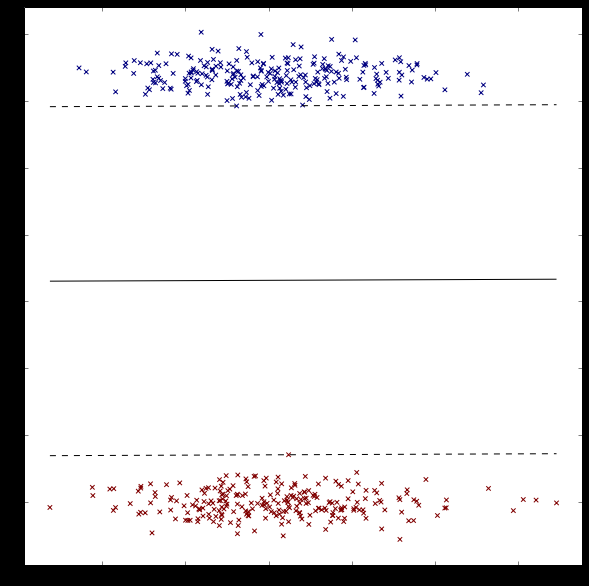
\includegraphics[width=\linewidth]{imgs/svm_linear.png}
\caption{Демонстрация SVM для линейно отделимых классов.}
\label{image:svm_linear}
\end{figure}
\par
В реальных задачах классификации не удается гарантировать линейную разделимость классов.
В этом случае вводятся новые переменные $\xi_i \ge 0$, характеризующие велечину ошибки 
на объектах $x_i$. Задача поиска разделяющей гиперплоскости формулируется в виде:
\[\begin{cases}
    \frac{1}{2}||w||^2+C\sum_{i=1}^n\xi_i \to \min_{w, b, \xi_i} \\
    y_i(wx_i-b)\ge 1-\xi_i,\ 1 \le i \le n \\
    \xi_i \ge 0,\ 1 \le i \le n,
\end{cases}\]
где $C$ параметр регуляризации, подбираемый для каждой задачи индивидуально.
\par
По теореме Каруша-Куна-Таккера эта система сводится к эквивалентной задаче
квадратичного программирования:
\[\begin{cases}
    -\sum_{i=1}^n \lambda_i + \frac{1}{2}\sum_{i=1}^n \lambda_i\lambda_j
    y_i y_j (x_i x_j) \to \min_\lambda \\
    0 \le \lambda_i \le C,\ 1 \le i \le n \\
    \sum_{i=1}^n \lambda_i y_i=0.
\end{cases}\]
\par
Дальнейшим развитием метода является использование ядрового перехода вместо
скалярного произведения $x_i$ и $x_j$. При такой замене переменных разделяющая 
гиперплоскость оказывается в пространстве большей размерности, чем исходное, поэтому
разделяющая гиперплоскость в исходном пространстве оказывается не обязательно линейной.
Стандартно в SVM используется радиальная базизная функция
в качестве ядра: $k(x_i, x_j)=e^{-\gamma||x_i-x_j||^2}$, с некоторым $\gamma>0$, 
подбирающимся индивидуально для каждой задачи.

\subsubsection{Байесовский классификатор.}

\par
Байесовский классификатор относит объект $x$ к классу $y$, 
вероятность которого для этого объекта максимальна:
\[
    y_i = \arg \max_{y\in\mathcal{Y}} P(y|x).
\]
По теореме Байеса:
\[
    P(y|x)=\frac{P(x|y)P(y)}{P(x)}.
\]
Знаменатель является константой, т.е. не влияет на результат классификации.
Далее, используя предположение о зависимости $x$ только от класса $y$, а не
от других объектов, перепишем числитель:
\[
    P(x_1, ..., x_n|y)P(Y) = P(Y)\prod_i P(x_i|y),
\]
где $x_i$ - признаковое описание объекта $x$. Итоговая формула классификатора имеет вид:
\[
    A(x)=\arg\max_{y\in\mathcal{Y}} P(y)\prod_i P(x_i|y).
\]

\subsubsection{Логистическая регрессия.}

\par
Логистическая регрессия является линейным алгоритмом классификации. Формула классификатора
имеет вид:
\[
    A(x) = sign(\sum_{i=1}^n w_i x_i - w_0),
\]
где $w$ - вектор весов классификатора, $w_0$ - порог принятия решения. Задача обучения
сводится к подбору вектора весов с помощью минимизации функции эмпирического риска
по всем $x^i$ из обучающей выборки $X$:
\[
    Q(w)=\sum_i ln(1+e^{-y^i(x^i, w)}) \to \min_w.
\]

\subsubsection{Градиентный бустинг.}

\par
Градиентный бустинг над решающими деревьями (Xgboost) 
\cite{xgboost} представляет алгоритм построения
классификатора на основе композиции решающих деревьев, так же как и случайный лес. 
Однако построение каждого следующего дерева учитывает уже построенные, а так же производную
оптимизируемой функции потерь. Данный подход позволяет сильно улучшить качество классификации.

\subsection{Настройка классификационной модели.}

\subsubsection{Оценка качества классификации.}

\par
Для оценки качества построенных классификационных моделей будет использован стандартный
для данных задач подход - скользящий контроль по $q$ блокам (q-fold cross validation).
Рассмотрим данный метод подробнее. 
Пусть $\mathcal{X}$ - множество описаний объектов, 
$\mathcal{Y}$ - конечное множество меток классов. Заданы конечная обучающая выборка
\[
    X^L=(x_i, y_i)_{i=1}^L \subset \mathcal{X} \times \mathcal{Y} 
\]
и алгоритм обучения - отображение $\mu$, которое
произвольной конечной обучающей выборке $X \subset \mathcal{X}$
ставит в соответствие алгоритм $A:\ X \to \mathcal{Y}$.
Тогда выборка разбивается случаным образом на $q$ непересекающихся блоков размеров
$k_1,...,k_q$:
\[
    X^L=X_1^{k_1} \cup ... \cup X_q^{k_q}
\]
таких, что $k_1+...+k_q=L$. Каждый блок по очереди становится контрольной опдвыборкой,
при этом алгоритм обучения строится по оставшися $q-1$ блокам. Критерий качества
определяется как средняя ошибка на контрольной подвыборке:
\[
    CV(\mu, X^L)=\frac{1}{q}\sum_{n=1}^q Q(\mu(X^L \setminus X_n^{k_n}),X_n^{k_n}),
\]
где $Q(A, X)$ - некоторый функционал качества алгоритма $A$.
\par
В данной работе нас интересует процент правильно определенных меток классов,
поэтому в качестве функционала качества берется точность (accuracy),
определяемую по формуле:
\[
    ACC=\frac{TP+TN}{P+N},
\]
где TP (true positives) - истинно положительные, TN (true negative) - истинно отрицательные,
P (positive) - положительные, N (negative) - отрицательные ответы.
\par
Отдельно стоит рассмотреть способы разбиения обучающей выборки на блоки для скользящего
контроля. Стандартным подходом является равновероятное отнесение каждого примера выборки
к одному из $q$ классов. Однако этот подход может завышать истинное значение функционала
качества, если нам интересна его оценка на выборке, пространственно удалённой от заданной
обучающей. Причиной такого завышения является непрерывность данных, т.е. вероятность 
одинакового ответа двух объектов увеличивается с уменьшением этого расстояния.
Для исследования этого эффекта будем использовать разбиения объектов выборки
(географических точек поверхности Земли) двумя способами: полосами и квадратными блоками,
см. рис. \ref{image:val_masks}. 
\begin{figure}[H]
\centering
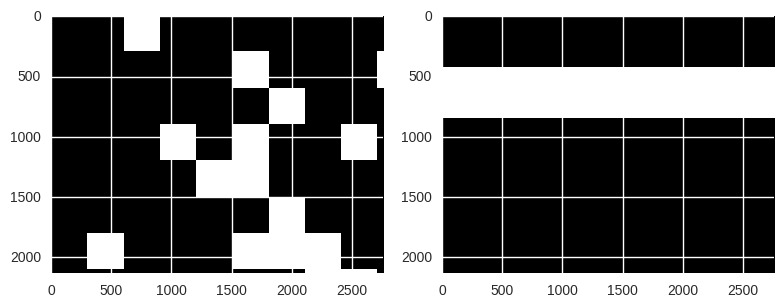
\includegraphics[width=\linewidth]{imgs/validation_masks.png}
\caption{Примеры маски скользящего контроля для разбиения квадратными блоками и полосами.}
\label{image:val_masks}
\end{figure}
Плюсом первого подхода является моделирование оценки качества на
пространственно удаленной территории. Однако для данной задачи при таком разбиении
не для всех классов будут попадать объекты и в обучающую и в контрольную подвыборки.
Этого недостатка не имеет метод с разбиением на квадратные блоки, при правильном
подборе размера стороны такого блока.
\par

\subsubsection{Оценка важности признаков.}

\par
Основным результатом решения задачи классификации, является построение модели, разделяющей
пространство на требуемые классы. Однако, на практике полезными оказываются и побочные результаты,
к которым относитя оценка важности признаков. Не все признаки, входящие в описание объектов
обучающей выборки оказываются одинкаово полезны для решения задачи классификации, и многие
модели позволяют провести численную оценку этой полезности. В данной работе используются методы
на основе деревьем принятия решения, входящие в алгоритмы: Random Forest и Xgboost. 
Для таких классификаторов существут 2 основных метода оценки важности признаков:
\begin{itemize}
    \item по количеству вхождений признака в вершины деревьев,
    \item по суммарной минимизации функции потерь.
\end{itemize}

\subsubsection{Подбор гиперпараметров модели.}

\par
Все используемые в работе классификационные модели имеют набор гиперпараметров, подбор которых
необходим для улучшения функционала качества. Оптимальные значения могут отличаться не только
для разных задач машинного обучения, но и на разных подзадачах, возникающих при классификации
типов почв по космическим снимкам. Будем использовать самый простой способ решения этой задачи - 
подбор гиперпараметров по заданнйо сетке. Основным недостатком этого метода являются
временные затраты в случае большого количества комбинаций параметров для перебора.
Однако для задач этой работы это оказывается не критичным. Опишем данный алгоритм подробнее.
\par
Пусть $p_1, ..., p_l$ - список настраеваемых параметров алгоритма обучения $\mu$.
Для каждого $p_i$ из них зададим список возможных значений $p_{i_{min}}, ..., p_{i_{max}}$,
где значения между максимальным и минимальным меняются либо с постоянным,
либо с логарифмическим шагом. Тогда оптимальными значениями $\bar{p_1}, ... \bar{p_l}$
определяются те, которые максимизируют оценку качества на скользящем контроле для
обучающей выобрки $X^L$:
\[
    \{\bar{p_i}\}_{i=1}^l=arg\max_{\{p_i\}} CV(\mu(\{p_i\}_{i=1}^l), X^L).
\]

\subsection{Данные для экспериментов.}

\par
Для исследований были взяты 34 фрагмента кадров спутников Landsat 5, 7, 8 
на территорию Павловского, Арсеньевского и Чернского районо Тульской области Российской Федерации.
Выбор именно этого спутника обусловлен тем, что программа Landsat является наиболее
продолжительным проектом по получению спутниковых снимков планеты. Так первый из спутников
был запущен в 1972 году, а последний на данный момент Landsat 8 - в 2013 году.
В данном исследовании нас интересует открытая поверхность почвы, которая на абсолютном
большинстве снимков исследуемой области покрыта облачным или снежным покровом.
По этой причине из нескольких сотен снимков за указанный промежуток времени были
отобраны только 35 штук, см. таб.\ref{table:scenes}.
\begin{table}[H]
\centering
\begin{tabu}{|l|l|l|}
    \hline
    \multicolumn{1}{|c|}{Номер} & \multicolumn{1}{c|}{Спутник} & \multicolumn{1}{c|}{Дата} \\
    \tabucline[1.5pt]{-} 
           1 & Landsat 5 & 16.05.1985 \\
    \hline 2 & Landsat 5 & 04.08.1985 \\
    \hline 3 & Landsat 5 & 03.05.1986 \\
    \hline 4 & Landsat 5 & 20.06.1986 \\
    \hline 5 & Landsat 5 & 06.07.1986 \\
    \hline 6 & Landsat 5 & 13.12.1986 \\
    \hline 7 & Landsat 5 & 29.10.1987 \\
    \hline 8 & Landsat 5 & 29.09.1988 \\
    \hline 9 & Landsat 5 & 27.05.1989 \\
    \hline 10& Landsat 5 & 14.07.1989 \\
    \hline 11& Landsat 5 & 14.05.1990 \\
    \hline 12& Landsat 5 & 12.07.1994 \\
    \hline 13& Landsat 5 & 29.08.1994 \\
    \hline 14& Landsat 5 & 02.04.1998 \\
    \hline 15& Landsat 5 & 20.05.1998 \\
    \hline 16& Landsat 7 & 06.10.1999 \\
    \hline 17& Landsat 7 & 17.05.2000 \\
    \hline 18& Landsat 7 & 04.05.2001 \\
    \hline 19& Landsat 7 & 23.05.2002 \\
    \hline 20& Landsat 7 & 27.08.2002 \\
    \hline 21& Landsat 7 & 14.10.2002 \\
    \hline 22& Landsat 7 & 26.05.2003 \\
    \hline 23& Landsat 5 & 23.09.2003 \\
    \hline 24& Landsat 5 & 14.08.2006 \\
    \hline 25& Landsat 5 & 17.08.2007 \\
    \hline 26& Landsat 5 & 09.08.2010 \\
    \hline 27& Landsat 5 & 08.05.2011 \\
    \hline 28& Landsat 5 & 27.07.2011 \\
    \hline 29& Landsat 5 & 28.08.2011 \\
    \hline 30& Landsat 8 & 29.03.2014 \\
    \hline 31& Landsat 8 & 20.08.2014 \\
    \hline 32& Landsat 8 & 29.09.2014 \\
    \hline 33& Landsat 8 & 23.10.2014 \\
    \hline 34& Landsat 8 & 16.03.2015 \\
    \hline 35& Landsat 8 & 06.07.2015 \\
    \hline
\end{tabu}
\caption{Список используемых снимков}
\label{table:scenes}
\end{table}

\par
Сами спутники, количество и качество их сенсоров претерпевали изменения на протяжении
программы Landsat. Для дальнейшего понимания приведем таблицу характеристик сенсоров
спутника на примере Landsat 8, см. таб. \ref{table:channels}
\begin{table}[H]
\centering
\begin{tabu}{|l|m{5cm}|l|}
    \hline
    \multicolumn{1}{|c|}{Номер} & \multicolumn{1}{c|}{Название} 
    & \multicolumn{1}{c|}{Разрешение} \\
    \tabucline[1.5pt]{-}
           1 & Побережья и аэрозоли (New Deep Blue) & 30 м \\
    \hline 2 & Синий (Blue) & 30 м \\
    \hline 3 & Зеленый (Green) & 30 м \\
    \hline 4 & Красный (Red) & 30 м \\
    \hline 5 & Ближний ИК (NIR) & 30 м \\
    \hline 6 & Ближний ИК (SWIR2) & 30 м \\
    \hline 7 & Ближний ИК (SWIR3) & 30 м \\
    \hline 8 & Панхроматический (PAN) & 15 м \\
    \hline 9 & Перистые облака (SWIR) & 30 м \\
    \hline 10& Дальний ИК (TIR1) & 100 м \\
    \hline 11& Дальний ИК (TIR2) & 100 м \\
    \hline
\end{tabu}
\caption{Список каналов Landsat 8}
\label{table:channels}
\end{table}

\par
Для каждой сцены представлены все каналы из таблицы, однако как будет показано ниже, не 
все из них одинаково информативны для задачи классификации типов почв. Основные признаки
будут связаны с тремя цветовыми каналами: Red, Blue, Green, а так же одним инфракрасным: Nir.
Размер всех исследуемых снимков равен 2132 на 2755 пикселей, что соответствует
63960 и 82650 метрам на поверхности Земли соответственно. Пример снимка Landsat 5 для
красного канала см. на рис. \ref{image:landsat_example}
\begin{figure}[H]
\centering
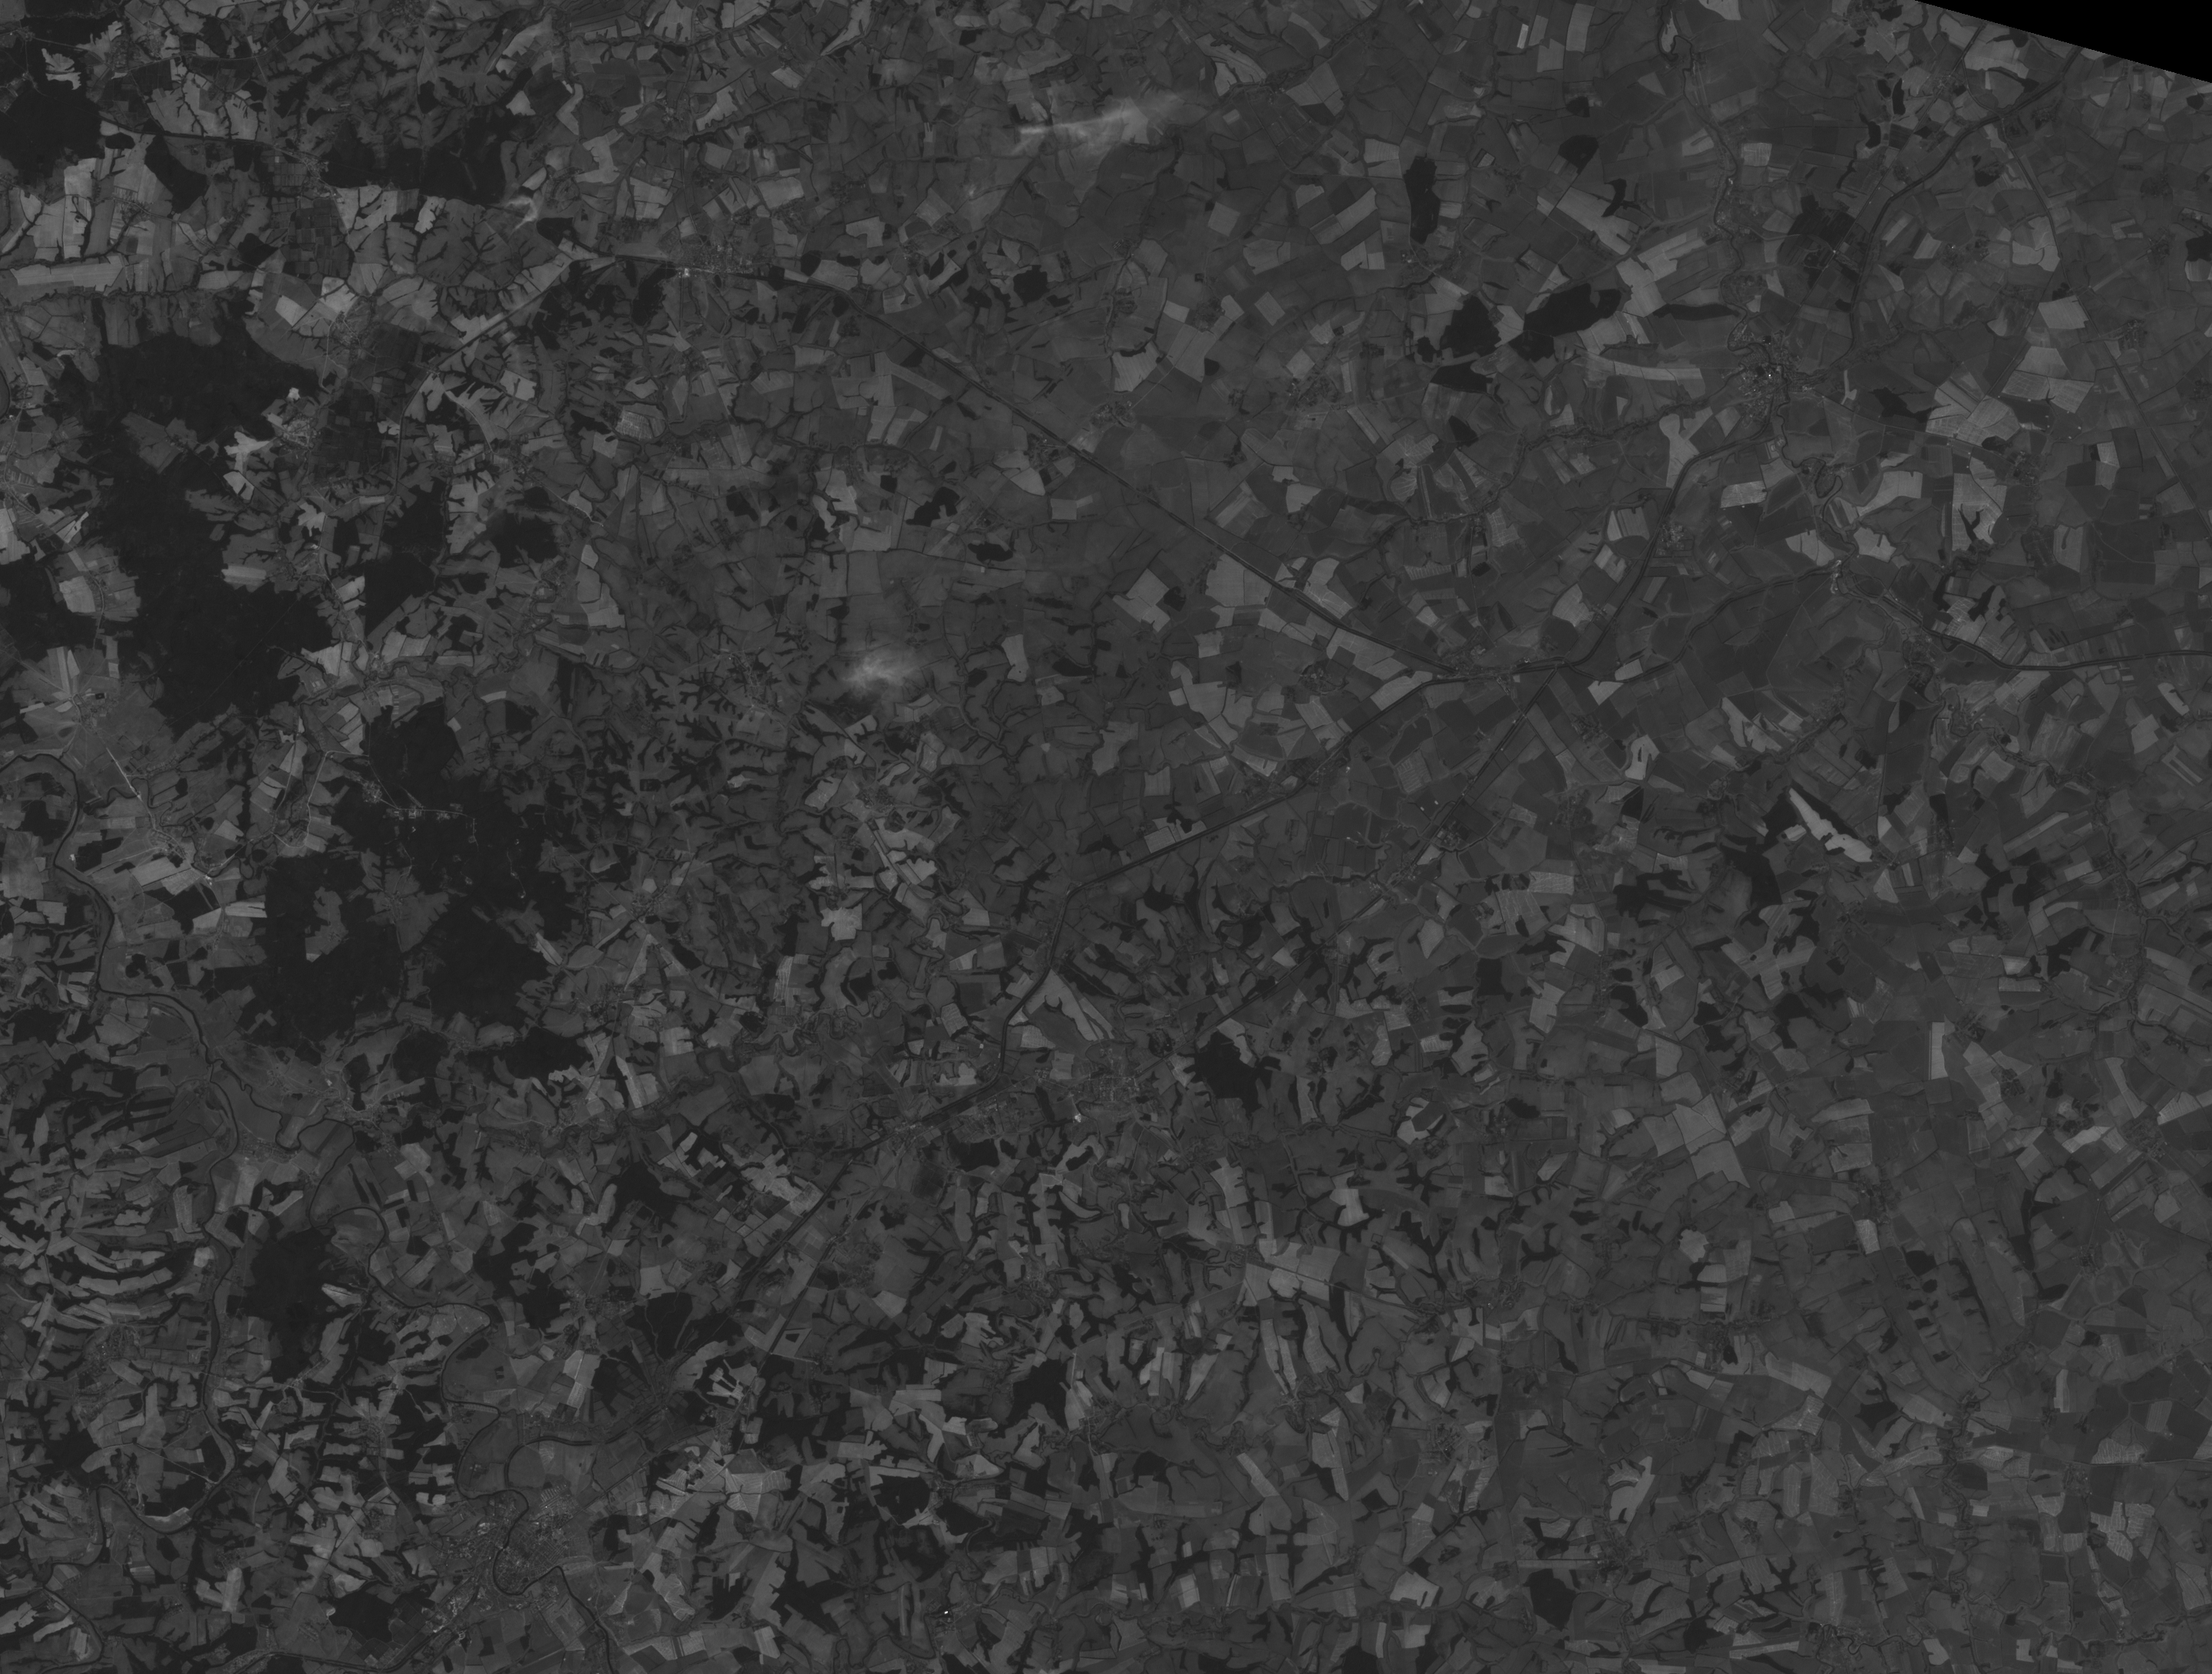
\includegraphics[width=\linewidth]{imgs/landsat_example.png}
\caption{Пример канала снимка Landsat}
\label{image:landsat_example}
\end{figure}
\par
Определим так же данные для извлечения меток классов, обязательных для задачи классификации.
В данной используются данные о распространении типов почв из 2 мест:
\begin{itemize}
    \item информация о почвенных разрезах из базы Научно-производственного института по 
        землеустройству, земельному кадастру и технической инвентаризации объектов
        недвижимости,
    \item почвенная карта исследуемой территории, предоставленная Почвенным институтом
        им. В.В. Докучаева.
\end{itemize}
Информация о 1761 почвенном разрезе содержит географические координаты каждого из них,
подробное описание типа почвы и сопутствующую информацию. Из почвенной карты удается
извлечь информацию о типе почв для 2503407 пикселей. Однако данные почвенной карты
имеют неточности, обусловленые отсутствием жестких границ между типами почвы. Поэтому хотя
для каждого пикселя и записана почва с максимальной по версии строящего карту человека
вероятностью, вероятность встретить там некоторые другие типы почв остается не нулевой.
Другой особенностью данных является иерархичность классификации типов почв.
В данной работе будут использованы типы почв с двух уровней иерархии классификации,
содержащие 3 и 9 классов соответственно, см. таб.\ref{table:soil-types}.
\begin{table}[H]
\centering
\begin{tabu}{|l|l|l|l|}
    \hline
    \multicolumn{2}{|c|}{Класс} & \multicolumn{2}{c|}{Тип почвы} \\
    \hline \multicolumn{1}{|c|}{1-3} & \multicolumn{1}{c|}{1-9} & 
    \multicolumn{1}{c|}{1-3} & \multicolumn{1}{c|}{1-9} \\ 
    \tabucline[1.5pt]{-} 1 & 1 & Дерново-подзолистые & Дерново-сильноподзолистые \\
    \hline 1 & 2 & Дерново-подзолистые & Дерново-среднеподзолистые \\
    \hline 1 & 3 & Дерново-подзолистые & Дерново-слабоподзолистые \\
    \hline 1 & 9 & Дерново-подзолистые & Д.-п. слабодифференцированные \\
    \hline 2 & 4 & Серые лесные & Светло-серые лесные \\
    \hline 2 & 5 & Серые лесные & Серые лесные \\
    \hline 2 & 6 & Серые лесные & Темно-серые лесные \\
    \hline 3 & 7 & Черноземы & Черноземы оподзоленные \\
    \hline 3 & 8 & Черноземы & Черноземы выщелоченные \\
    \hline
\end{tabu}
\caption{Типы почв}
\label{table:soil-types}
\end{table}

\subsection{Модель линии почвы.}

\par
Понятие линия почвы (ЛП) введено и описано в статье \cite{soil-line-4}, как нижняя граница
треугольной области представления снимка в спектральном пространстве Red-Nir.
Переход в указанное спектральное пространство является отображением значений каналов Red и Nir
каждого пикселя в двумерную декартову систему координат, по осям которой отложены эти значения,
см. рис. \ref{image:soil_line_model}.
\begin{figure}[H]
\centering
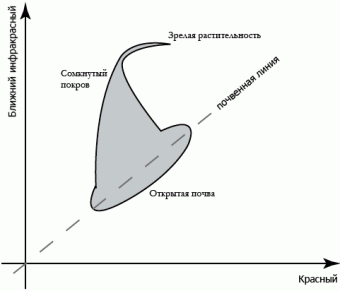
\includegraphics[width=\linewidth]{imgs/soil_line_model.png}
\caption{Модель линии почвы}
\label{image:soil_line_model}
\end{figure}
\par
В таком виде линия почвы отделяет область плоскости Red-Nir, соответствующую голой почве, от
остальной части, соответствующей сомкнутому растительному покрову и другим объектам.
Классическая ЛП представляется в виде вытянутого эллипса, разделяющего положительный квадрант
спектральной плоскости Red-Nir на 2 примерно равные части.
\par
С другой стороны, линия почвы является частью математического аппарата расчета
вегетационных индексов. В этом случае линия почвы определяется не как область спектрального
пространства, а как прямая в нем же, задающаяся классическим уравнениес с коэффициентами
$a$ и $b$. В этих подходах линия почвы определяется либо константно, например 
$a=1,\ b=0$ для вегетационного индекса NDVI, либо как прямая, ниже которой нет ни 
одной точки в пространстве Red-Nir \cite{soil-line-5}. Тогда область голой почвы
определяется, как полоса фиксированной ширины над линией почвы.
\par
В приведеных выше вариантах трактовки понятия линии почвы она является характеристикой
конкретного кадра космической съемки. В данной работе используется также линия почвы 
временная (ЛПВ), введенная в \cite{rukhovich-1}, см. \ref{image:soil_line_time}. 
\begin{figure}[H]
\centering
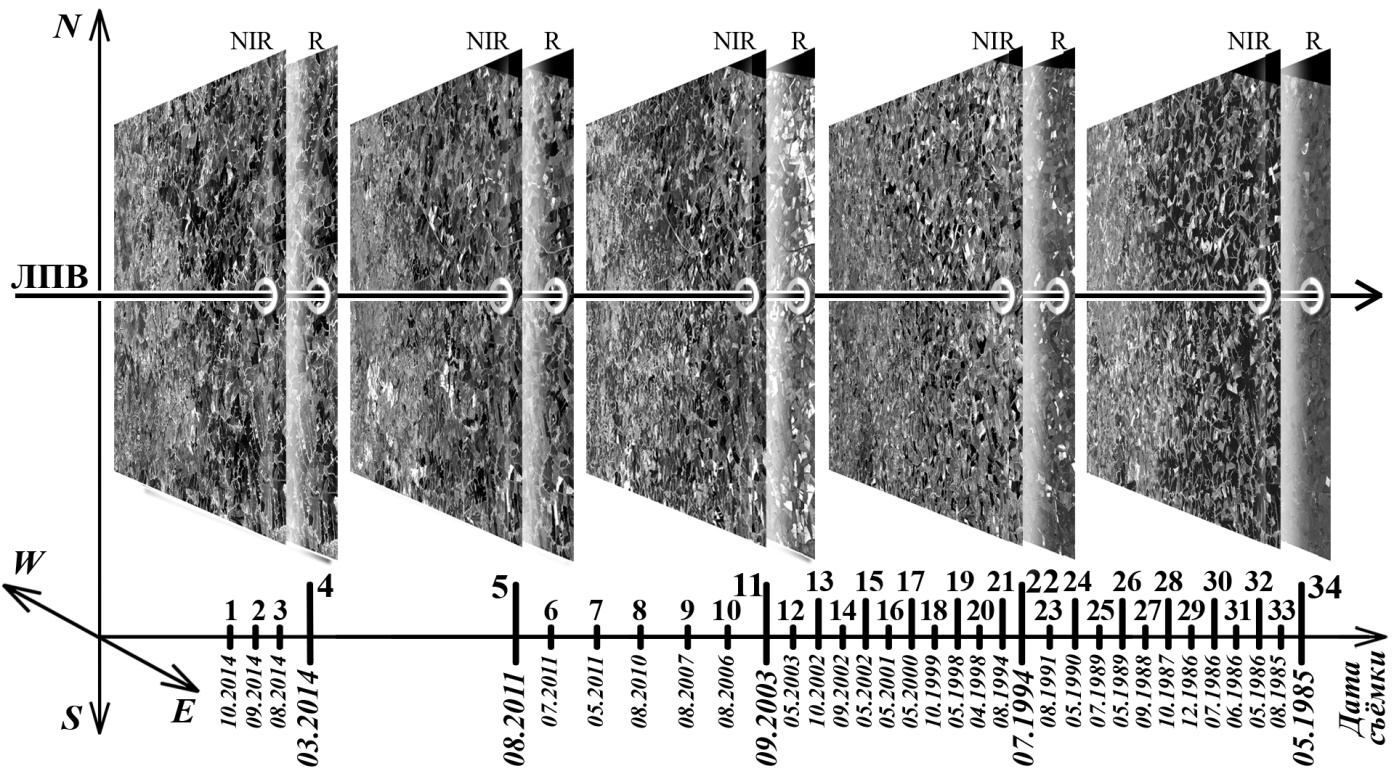
\includegraphics[width=\linewidth]{imgs/soil_line_time.png}
\caption{Линия почвы временная}
\label{image:soil_line_time}
\end{figure}
В этом случае линия почвы является совокупностью спектральных значений Red-Nir,
которые принимает во времени однородный участок почвенного покрова, при условии, что
спектральные характеристики получены для открытой поверхности.

\subsection{Предобработка снимков.}

\subsubsection{Фильтрация снимков.}

\par
Для задачи классификации типов почв по набору космических снимков не все пиксели этих снимков
имею одинковую пользу, а некоторые значения мешают построению признаковых описаний. В идеале
для решения задачи необходимо использовать только пиксели, попадающие в облаcть голой почвы
на каждом из снимков. В область голой почвы не входят:
\begin{itemize}
    \item некоторые элементы ландшафта (реки, озера),
    \item снежный покров,
    \item облачный покров,
    \item области вегетирующей в момент съемки растительности,
    \item неприродные объекты (дороги, здания).
\end{itemize}
В данной работе для построения области голой почвы, была использована
модель спектральной окрестности линии почвы, описанная выше в разделе 3.4.
\par
Построение алгоритма выделения спектральной окрестности линии почвы по распределению 
значений в каналах Red и Nir лежит за пределами исследований данной работы. Известные на данный
момент автоматические алгоритмы построения линии почвы, 
описанные, например, в \cite{soil-line-5},
оказываются не применимы в данной задаче, т.к. окрестность не дадается не самим уравнением линии
почвы, ни нимерьшими значениями Red при фиксированных Nir, как предлагается в этой статье.
По этим причинам данный шаг предобработки спутниковых снимков оставлен в полуавтоматическом режиме,
т.е. спектральная окрестность линии почвы выделяется экспертом почвоведом по графику распределения
значений, см. рис. \ref{image:soil_line_plot}.
\begin{figure}[H]
\centering
    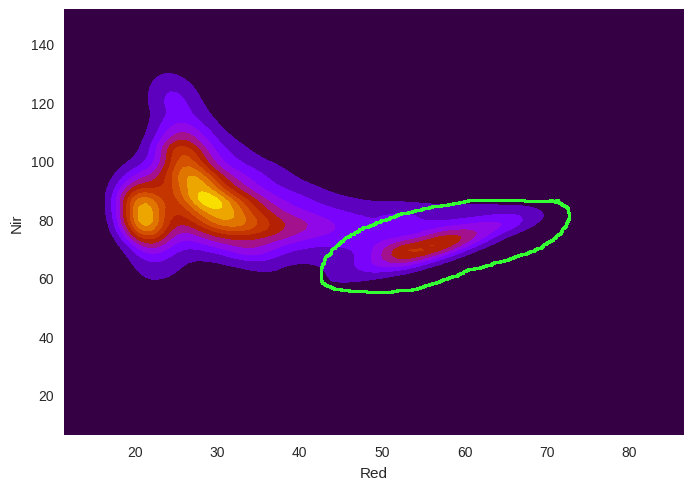
\includegraphics[width=\linewidth]{imgs/soil_line_plot.png}
\caption{Пример выделения области голой почвы}
\label{image:soil_line_plot}
\end{figure}
\par
Заметим так же, что выделенная окрестность однозначно отображается в пространство объектов,
т.е. георафических точек поверхности Земли. Поэтому по той же пространственной области
фильтруются и другие каналы спутниковых снимков: Green, Blue и т.д.

\subsubsection{Нормализация снимков.}

\par
Как было указано в разделе 3.3 данные для исследований содержат спутниковые снимки
одной области за более 15 лет. Такой массив данных порождает проблемы нормализации этих снимков,
т.к. статистические характеристики распределений значений в их каналах существенно различаются.
Эти различия объясняются следующими основными факторами:
\begin{itemize}
    \item различия сенсоров на спутниках разных версий,
    \item различия примененных на спутниках постобработок значений,
    \item различия условий освещения и параметров атмосферы в момент съемки.
\end{itemize}
\par
Единого метода нормализации космических снимков не существует, и для каждой задачи он
подбирается индивидуально. В статье \cite{rukhovich-2} исследуются следующие методы нормализации
для уменьшения отклонений кусочно-линейных аппроксимаций спектральной окрестности 
разных снимков друг от друга:
\begin{itemize}
    \item классическая нормализация (вычитание математического ожидания и деление на дисперсию),
    \item последовательное применение поворота и сдвига,
    \item последовательное применение атмосферной коррекции и сдвига,
    \item атмосферная коррекция,
    \item сдвиг,
    \item поворот,
\item исходные данные (без нормализации).
\end{itemize}
Авторы приходят к выводу, что для данной задачи наилучшие результаты 
показывает классическая нормализация. В разделе 4 будет проведено сравнение основных
типов нормализации в применении к решению задачи классификации.

\subsubsection{Усреднение снимков.}

Важной проблемой при обработке цифровых снимков является подавление шумов,
неизбежно возникающих из-за несовершеноства снимающего сенсора и условий съемки.
Для подавления шумов используются такие методы как гауссовский, медианный или билатеральный
фильтр. В данной работе будет использоваться медианный фильтр, т.к. он не порождает новых значений,
а заменяет значение пикселя на медианут значений его пространственной окрестности.
Единственным параметром медианной фильтрации является радиус в пикселях пространственной
окрестности. Влияние радиуса усреднения на качество решения задачи классификации будет рассмотрено
а разделе 4.

\subsection{Итоговое признаковое описание объектов.}

Признаковое описание для каждой исследуемой географической точки строится по всем накрывающим
её разноврменным космическим снимкам, прошедших 3 стадии предобработки: фильтрацию,
нормализацию и усреднение. В данной работе признаки берутся из множества статистических
характеристик распределений значений 4 цветовых каналов: Red, Nir, Green, Blue. Дополнительно
признаками являлются коэффициент наклона линии почвы временной и доля выборки, не принадлежащая
маске фильтрации. Приведем формулы вычисления всех 18 используемых признаков. Обозначим 
$M$ - множество индексов снимков, значения которых в данной точке не входит в маску фильтрации.
\begin{align*}
    E_{red} &= \frac{1}{|M|}\sum_{i \in M} red_i \\
    STD_{red} &= \frac{1}{|M|}\sum_{i \in M} (red_i - E_{red})^2 \\
    MIN_{red} &= \min_{i \in M} red_i \\
    MAX_{red} &= \max_{i \in M} red_i \\
\end{align*}
\begin{align*}
    E_{nir} &= \frac{1}{|M|}\sum_{i \in M} nir_i \\
    STD_{nir} &= \frac{1}{|M|}\sum_{i \in M} (nir_i - E_{nir})^2 \\
    MIN_{nir} &= \min_{i \in M} nir_i \\
    MAX_{nir} &= \max_{i \in M} nir_i \\
\end{align*}
\begin{align*}
    E_{green} &= \frac{1}{|M|}\sum_{i \in M} green_i \\
    STD_{green} &= \frac{1}{|M|}\sum_{i \in M} (green_i - E_{green})^2 \\
    MIN_{green} &= \min_{i \in M} green_i \\
    MAX_{green} &= \max_{i \in M} green_i \\
\end{align*}
\begin{align*}
    E_{blue} &= \frac{1}{|M|}\sum_{i \in M} blue_i \\
    STD_{blue} &= \frac{1}{|M|}\sum_{i \in M} (blue_i - E_{blue})^2 \\
    MIN_{blue} &= \min_{i \in M} blue_i \\
    MAX_{blue} &= \max_{i \in M} blue_i \\
\end{align*}
\begin{align*}
    A_{soil\_line} &= \frac{|M|\sum_{i \in M} red_i nir_i - 
                            \sum_{i \in M} red_i \sum_{i \in M} nir_i}
                           {|M|\sum_{i \in M} red_i^2 - 
                            \left(\sum_{i \in M} red_i\right)^2} \\
    N_{mask} &= |M|
\end{align*}

\section{Эксперименты.}

\subsection{Используемая вычислительная система.}

Все вычисления производились на вычислительной системе с процессором Intel Core i5 2.8 ГГц,
16 Гб оперативной памяти и операционной системой Ubuntu 16.04. Все эксперименты и
сопутствующая обработка данных были запрограммированы на языке Python 3.5 
\cite{python} с использованием
библиотек машинного обучения scikit-learn 0.18.1 \cite{sklearn} и 
xgboost 0.6 \cite{xgboost}.

\subsection{Классификация по данным почвенных разрезов.}

\par
В данном разделе будут показаны результаты решения задачи классификации при использовании
данных для обучающей выборки только из информации о почвенных разрезах.
\par
Для выбора оптимального классификатора была измерена точность предсказаний всех
моделей, описанных в разделе 3.1, см. таб. \ref{table:cuts_clf}.
На вход каждому классификатору поданы данные с одинаковой
предобработкой: классическая нормализация и усреднение по радиусу 50 пикселей.
\begin{table}[H]
\centering
\begin{tabu}{|l|l|l|}
    \hline
    \multicolumn{1}{|c|}{Классификатор} & \multicolumn{1}{c|}{Точность, 9 классов} 
    & \multicolumn{1}{c|}{Точность, 3 класса} \\
    \tabucline[1.5pt]{-} 
           kNN & 54.9\% & 88.5\% \\
    \hline Random Forest & 60.5\% & 91.2\% \\ 
    \hline SVM & 59.1\% & 90.2\% \\
    \hline Bayesian & 54.1\% & 85.9\% \\
    \hline Log Regression & 53.2\% & 90.0\% \\
    \hline Xgboost & 59.7\% & 91.0\% \\
    \hline
\end{tabu}
\caption{Сравнение классификаторов.}
\label{table:cuts_clf}
\end{table}
\par
Для достижения максимальной точности некоторые гиперпараметры классификаторов подбирались
с помощью подхода, описанного в разделе 3.2.3. Так при разбиении на 9 классов 
для метода ближайших соседей оптимальным числом соседей оказалось 20; 
для машины опорных векторов - коэффициент регуляризации 1000 и 
степенной показатель гауссовского ядра 0.001; для случайного леса - количество деревьев 300;
для градиентного бустинга - количество деревьев 200, скорость обучения 0.3, максимальная 
глубина дерева 7. В итоге SVM, Random Forest и Xgboost дают точность на скользящем контроле
выше 59\% и лучшая точность 60.5\% достигается классификатором Random Forest.
\par
При разбиении на 3 класса для метода ближайших соседей оптимальным числом соседей оказывается
3; для метода опорных векторов коэффициент регуляризации 50 
и степенной показатель гауссовского ядра 0.1, количество деревьев для градиентного бустинга
и случайного леса равняется 200. Все алгоритмы показывают отличную точность разбиения
на 3 класса - около 90\%. А Xgboost и Random Forest достигают точности выше 91\%.
\par
Далее были проведены эксперименты с различными типами нормализации спутниковых снимков,
описанные в разделе 3.5.2 и радиусами медианной фильтраницей снимков, описанной в разделе
3.5.3. Сравнение классической (mean+std) нормализации, атмосферной коррекции (rad+refl) и
подхода без нормализации преведено в таблице \ref{table:cuts_norm}.
\begin{table}[H]
\centering
\begin{tabu}{|l|l|l|}
    \hline
    \multicolumn{1}{|c|}{Нормализация} & \multicolumn{1}{c|}{Точность, 9 классов} & 
    \multicolumn{1}{c|}{Точность, 3 класса} \\
    \tabucline[1.5pt]{-}
           mean+std & 60.5\% & 90.6\% \\
    \hline none & 59.5\% & 89.4\% \\
    \hline rad+refl & 63.1\% & 91.2\% \\
    \hline
\end{tabu}
\caption{Сравнение нормализаций.}
\label{table:cuts_norm}
\end{table}
\par
Для сочетания классификатора и нормализации, показывающих лучшую точность проведено
исследование влияния радиуса усреднения на итоговую точность, см. рис.
\ref{image:cuts_radius}.
\begin{figure}[H]
\centering
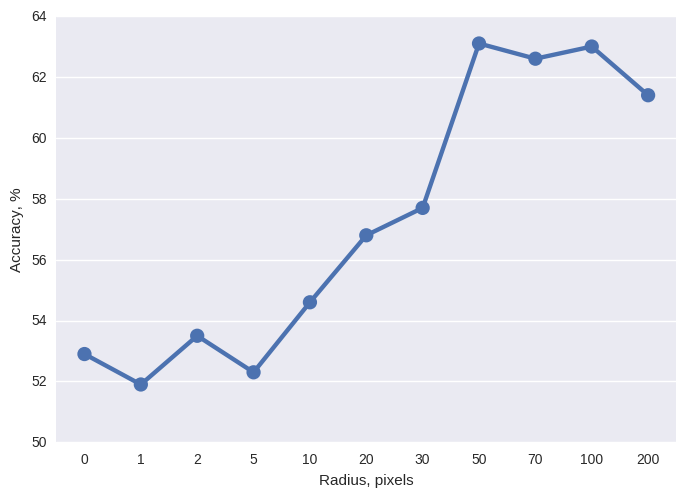
\includegraphics[width=\linewidth]{imgs/cuts_radius.png}
\caption{Сравнение радиусов усреднения.}
\label{image:cuts_radius}
\end{figure}
Из результатов двух экспериментов выше следует, что тип нормализации влияет на точность не сильно,
но при нормализации на коэффициенты атмосферной коррекции достигается 63\%. Радиус усреднения
сырых снимков влияет на точность существенно: без усреднения - 52\%, 
при радиусе 50 пикселей - 63\%.
\par
Также были проведены исследования важности признаков, методами описанными в разделе 3.2.2.
Важности признаков, оцененные для обученного Xgboost классификатора показаны на рис. 
\ref{image:cuts_importance}.
\begin{figure}[H]
\centering
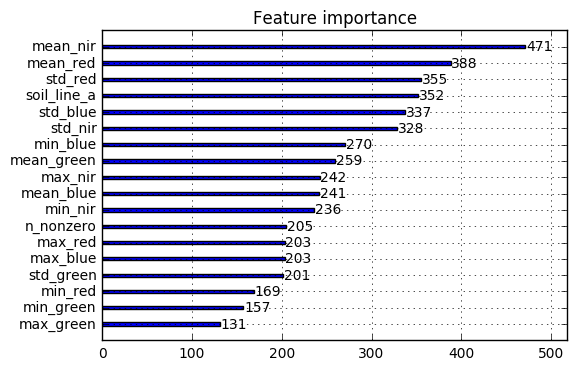
\includegraphics[width=\linewidth]{imgs/cuts_importance.png}
\caption{Сравнение важности признаков.}
\label{image:cuts_importance}
\end{figure}
Эти результаты показывают, что красный и ближний инфракрасный канал содержут больше информации
о типе почве, чем остальные. А параметры описанной в разделе 3.4 линии почвы временной:
среднее по горизонтальной и вертикальной осям а также коэффициент наклона являются тремя
важнейшими признаками для задачи классификации типов почв по космическим снимкам.

\subsection{Классификация по данным почвенной карты.}

Все аналогичные эксперименты были проведены и для обучения по данным классов, полученным
из почвенной карты. Сравнение показателей раличных классификационных моделей при разбиении
на 3 и 9 классов приведено в таблице \ref{table:map_clf}.
\begin{table}[H]
\centering
\begin{tabu}{|l|l|l|}
    \hline
    \multicolumn{1}{|c|}{Классификатор} & \multicolumn{1}{c|}{Точность, 9 классов} 
    & \multicolumn{1}{c|}{Точность, 3 класса} \\
    \tabucline[1.5pt]{-} 
           kNN & 72.9\% & 94.6\% \\
    \hline Random Forest & 78.9\% & 95.2\% \\ 
    \hline SVM & 70.2\% & 95.6\%\\
    \hline Bayesian & 52.5\% & 89.1\% \\
    \hline Log Regression & 56.8\% & 90.1\% \\
    \hline Xgboost & 80.1\% & 95.7\% \\
    \hline
\end{tabu}
\caption{Сравнение классификаторов.}
\label{table:map_clf}
\end{table}
Все измерения проведены при одинаковом методе получения обучающей выборки:
классическая нормализация, усреднение снимков по радиусу 50 пикселей, выбор 10000 случайных
точек карты для обучения. Гиперпараменты классификаторов также были подобраны перебором по сетке
при: проверке качества скользящим контролем. Здесь точность разбиения на 9 классов достигается 
порядка 80\%, а на 3 класса - 95\%. Лучшим классификатором оказывается Xgboost,
показывающий точности 80.1\% и 95.7\% соответственно. Важным свойством данного результата
является небольшой размер обучающей выборки по сравнению со всей картой, т.к. для достижения
отличных точностей требуется размер обучающей выборки, равный всего 0.3\% от 
количества точек самой карты.
\par
В таблице \ref{table:map_norm} приведены результаты сравнения 3 разных нормализаций для
лучшего из классификаторов, полученного выше. 
\begin{table}[H]
\centering
\begin{tabu}{|l|l|l|}
    \hline
    \multicolumn{1}{|c|}{Нормализация} & \multicolumn{1}{c|}{Точность, 9 классов}
    & \multicolumn{1}{c|}{Точность, 3 класса} \\
    \tabucline[1.5pt]{-}
           mean+std & 80.1\% & 95.3\% \\
    \hline none & 78.9\% & 95.1\% \\
    \hline rad+refl & 81.2\% & 95.7\%\\
    \hline
\end{tabu}
\caption{Сравнение нормализаций.}
\label{table:map_norm}
\end{table}
Тип нормализации не оказывает сильного влияния на результирующую тоность, однако как и 
при обучении по данным почвенных разрезов лучшей оказывает нормализация на коэффичиенты
атмосферной коррекции.
\par
Сравнение влияния радиуса усредления сырых снимков на точность классификации, приведенное на
рис. \ref{image:map_radius}, также подтверждает, что для аднной задачи лучшим радиусом оказыватся -
50 пикселей.
\begin{figure}[H]
\centering
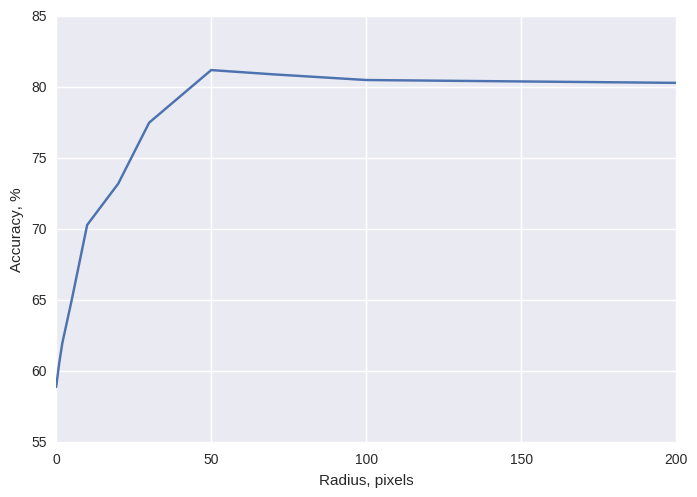
\includegraphics[width=\linewidth]{imgs/map_radius.png}
\caption{Сравнение радиусов усреднения.}
\label{image:map_radius}
\end{figure}
\par
Результаты оценки важности признаков для классификатора Xgboost показаны на рис. 
\ref{image:map_importance}. Как и при обучении по почвенным разрезам, тремя важнейшими
признаками оказывают параметры линии почвы временной: среднее красного и ближнего инфракрасного
каналов, а также её коэффициент наклона.
\begin{figure}[H]
\centering
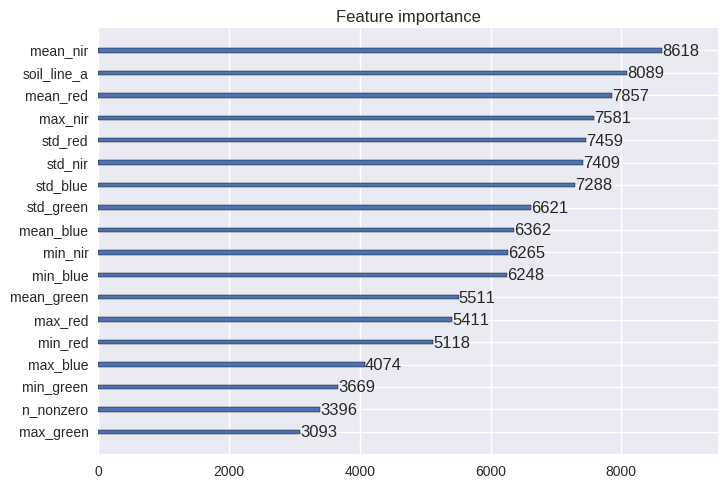
\includegraphics[width=\linewidth]{imgs/map_importance.png}
\caption{Сравнение важности признаков.}
\label{image:map_importance}
\end{figure}
\par
Решающее влияние на точность классификации при использовании почвенной карты территории оказывает
количество объектов, выбранных для обучающей выборки. Графики качества при разных
размерах обучающей выборки для 3 типов валидации для случаев разбиения на 9 и 3 класса
приведены на рис. \ref{image:map_val_9} и рис. \ref{image:map_val_3}.
\begin{figure}[H]
\centering
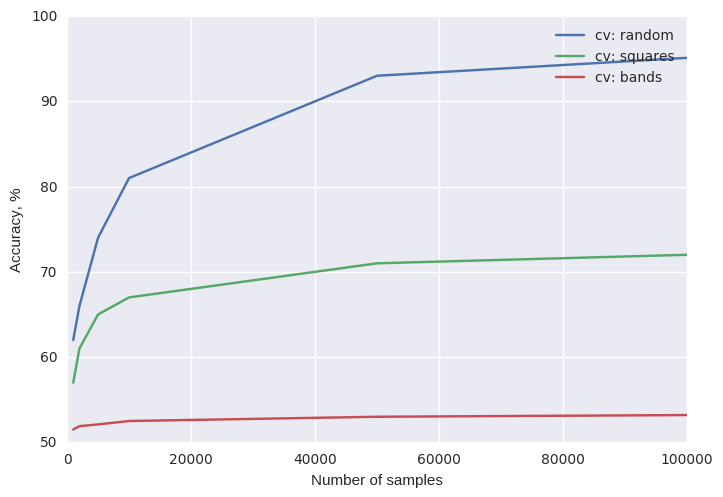
\includegraphics[width=\linewidth]{imgs/map_validations_9_classes.png}
\caption{Сравнение размеров обучающей выборки, 9 классов.}
\label{image:map_val_9}
\end{figure}
\begin{figure}[H]
\centering
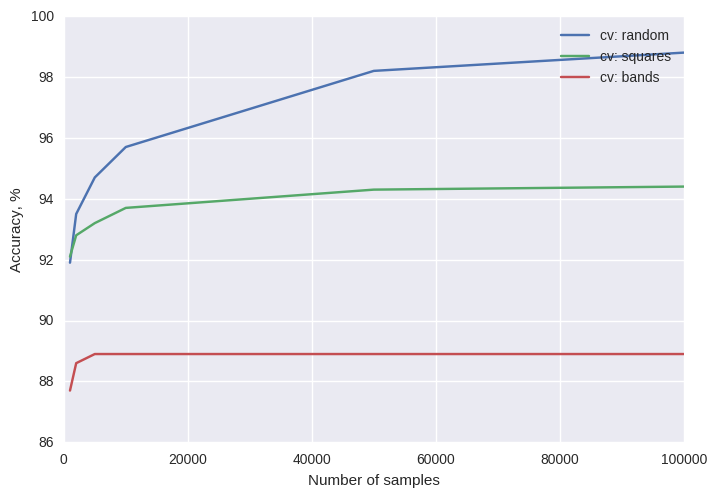
\includegraphics[width=\linewidth]{imgs/map_validations_3_classes.png}
\caption{Сравнение размеров обучающей выборки, 3 класса.}
\label{image:map_val_3}
\end{figure}
Результаты сильно отличаются в зависимости от типа разбиения выборки при валидации.
При стандартном скользящем контроле, т.е. когда все объекты обучающей и тестовой частей
выбираются их всей выборки случайно, точность для 9 и 3 классов достигает 94\% и 99\%.
Однако такие высокие числа, как было описано в разделе 3.2.1, объясняются тем, что ответы
для объектов зависят от расстояния между ними. Скользящий контроль с выбиранием тестовой части
выборки из фиксированной полосы всех снимков, показывает горадно более плохие результаты, а 
ведь именно такой контроль позволяет говорить о переносимости обученного классификатор а на 
другие территории. Для 9 классов эта цифра всего 50.0\%, а для 3 классов достигает
88.9\%, что является неплохим результатом. Валидация с разбиением выборки на 
случайные квадратные блоки, показывает, как и ожидалось, результаты между
2 другими типами валидации, это 71.8\% и 94.4\% для 9 и 3 классов соответственно.

\section{Заключение.}

\par
В работе проведено исследование применимости стандартных алгоритмов решения задачи классификации
для разделения поверхности, заданной набором развонвременных космических снимков, на регионы,
обладающие почвенной интерпретацией. Показана целесообразность использования коллекции
разновременных снимков, а также информативность коэффициентов линии почвы временной для
данной задачи классификации. Исследовано слияние типа нормализации сырого снимка
и радиуса его усреднения на итоговое качество классификации.
\par
При использовании в обучающей выборки данных почвенных разрезов достигнуты точности 63\% и 
91.2\% для разбиения на 9 и 3 класса соответственно. При обучении по данным почвенной карты
для трёх типов валидации: случайной, блоками и полосами достигнуты точности 94\%, 71\% и 50\%
при разбиении на 9 классов и 98\%, 94\%, 89\% при разбиении на 3 класса.
\begin{thebibliography}{9}
    \bibitem{rukhovich-1} 
        Rukhovich, D.I., Rukhovich, A.D., Rukhovich, D.D. et al, 
        "The informativeness of coefficients a and b of the 
        soil line for the analysis of remote sensing materials",
        Eurasian Soil Sc. (2016) 49.
    \bibitem{rukhovich-2}
        Rukhovich, D.I., Rukhovich, A.D., Rukhovich, D.D. et al, 
        "The Application of the Piecewise Linear Approximation
        to the Spectral Neighborhood of Soil Line for the Analysis
        of the Quality of Normalization of Remote Sensing Materials",
        Eurasian Soil Sc. (2017) 50.
    \bibitem{rukhovich-3}
        Rukhovich, D.I., Rukhovich, A.D., Rukhovich, D.D. et al, 
        "Maps of Averaged Spectral Deviations from Soil Lines
        and Their Comparison with Traditional Soil Maps",
        Eurasian Soil Sc. (2016) 49.
    \bibitem{salt-1}
        Габченко М.В., "Изучение структуры почвенного покрова территории солонцовых
        комплексов северного прикаспия по данным многозональной съемки", 
        Известия Россияской академении наук, серия географическая (2008) 3.
    \bibitem{salt-2}
        Конюшкова М.В., "Цифровое картографирование почв солонцовых комплексов
        северного прикаспия" (2014)
    \bibitem{soil-line-1}
        Украинский П.А., Землякова А.В., "Определение параметров почвенной линии
        для автоматического распознавания открытой поверхности почвы на космических
        снимках", Международный журнал прикладных и фундаментальных исследований
        (2014) 9.
    \bibitem{soil-line-3}
        Кирьянова Е.Ю., Савин И. Ю., "Линия почв как индикатор неоднородности
        почвенного покрова", Современные проблемы дистанционного зондирования
        Земли из космоса (2011) 8.
    \bibitem{soil-line-4}
        Черный С.Г., Абрамов Д.А., "Определение параметров линии почв черноземов
        правобережной Украины с помощью спектральных спутниковых снимков Ландсат-7",
        "Gruntoznavstvo" (2013) 14.
    \bibitem{soil-line-5}
        Kauth R.J., Thomas G.S., "The tasseled cap - a graphic description of the
        spectral-temporal developement of agricultural crops as seen by Landsat",
        Proceedings of the symposium on machine processing of remotely sensed data (1976)
    \bibitem{soil-line-6}
        Fox G.A., Sabbagh G.J. et al, "An automated soil line identification routine
        for remotely sensed images", Soil-science society of America (2004) 68.
    \bibitem{soil-line-7}
        Nanni M.R. et al, "Soil surface spectral data from Landsat imagery for soil class
        discrimination", Acta Scientiarum Agronomy (2012) 34.
    \bibitem{python}
        Python Software Foundation, "Python Language Reference, 
        version 3.5". Available at http://www.python.org
    \bibitem{sklearn}
        Pedregosa F. et al, "Scikit-learn: Machine Learning in Python",
        Journal of Machine Learning Research (2011) 12.
    \bibitem{xgboost}
        Chen T., Guestrin C., "XGBoost: A Scalable Tree Boosting System" (2016).
\end{thebibliography}

\end{document}
